\chapter{Design}
The application comprises the system design, architecture adopted, approach followed and the database used with a brief justification on why and how they are incorporated. 

\section{Approach}
The Approach followed for developing this application from scratch is a step-by-step practise which are as follows:
    \begin{itemize}
        \item Wireframe Diagrams
        \item H2 Database Installation 
        \item Initial Springboot setup
        \item Installed Angular modules and implemented design               
        \item Agile approach
    \end{itemize}
    
    
    
   Let's see how it evolved one-by-one and the reason for adopting the model. 
\begin{enumerate} 

    \item \textbf{Wireframe Diagrams}\newline
     Wireframe diagrams act as a key step to begin any web development and get consent from the clients regarding the requirements on how it might look on screen. So it is considered more vital for any development process. Wireframes provides the layout for the final product and it acts as a rough sketch for the application\cite{ngo2019android}.
     So, I have completed the requirements analysis phase and then designed the wireframe diagrams for getting approval from the Professor for proceeding with the initial designs and ideas which further evolved on development.
     
     So, here are some of the screenshots of wireframe diagrams in the intial phase of design.\newline
     
   \begin{figure}[h!]
    \begin{multicols}{2}
    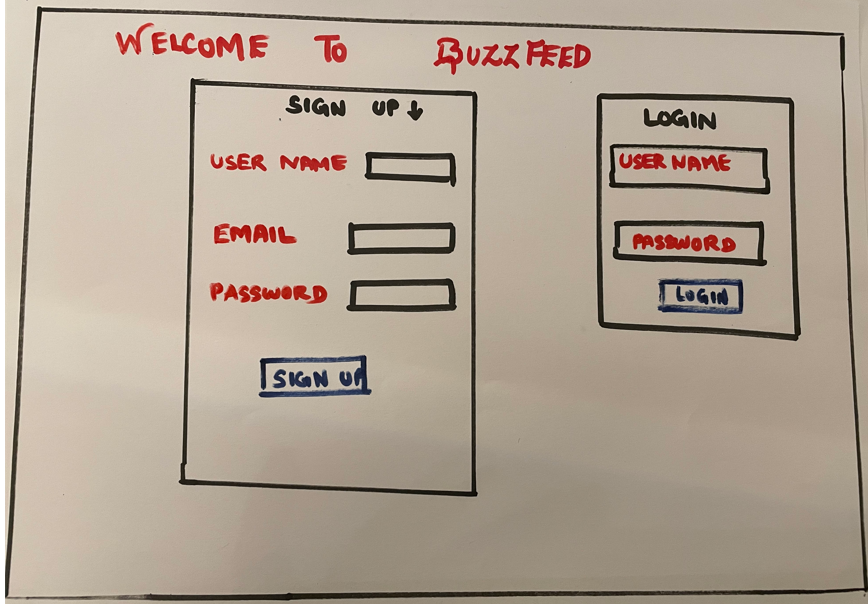
\includegraphics[width=\linewidth]{images/signup.png}\par 
    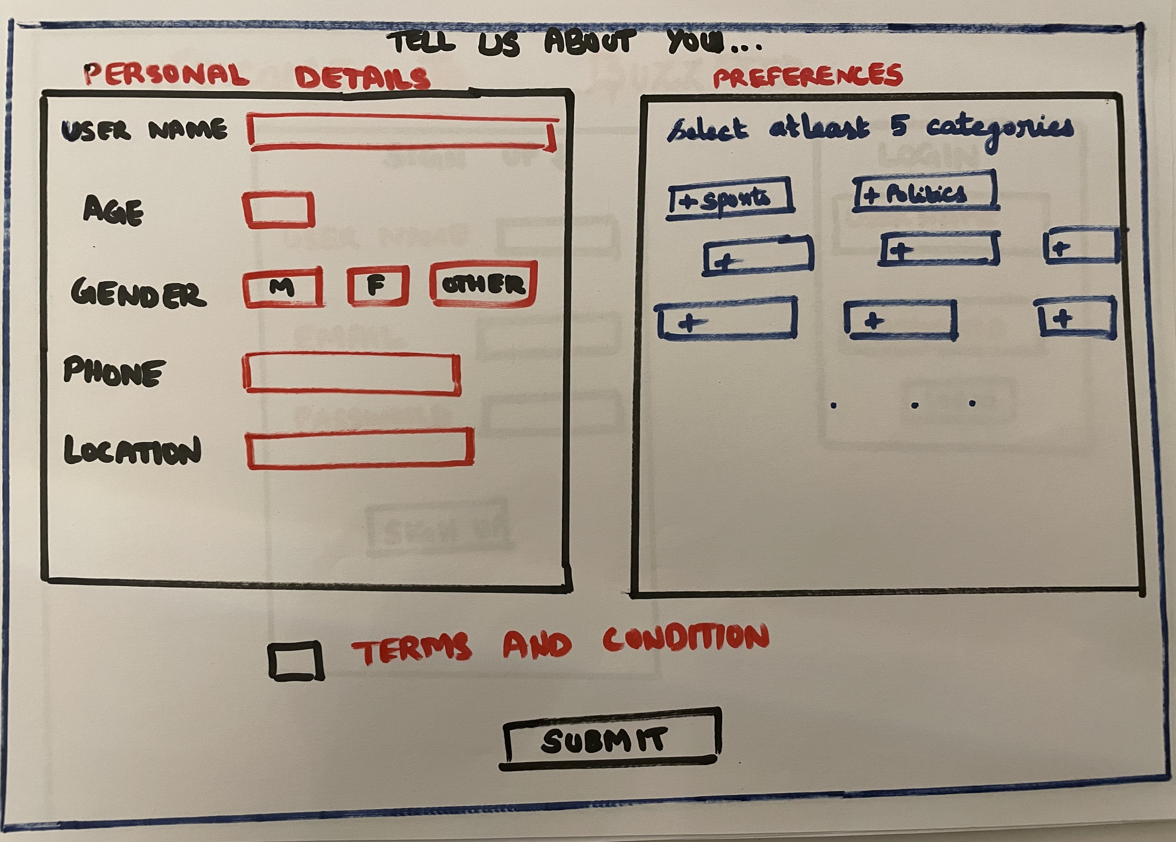
\includegraphics[width=\linewidth]{images/userdetails-signup.png}\par 
    \end{multicols}
\begin{multicols}{2}
    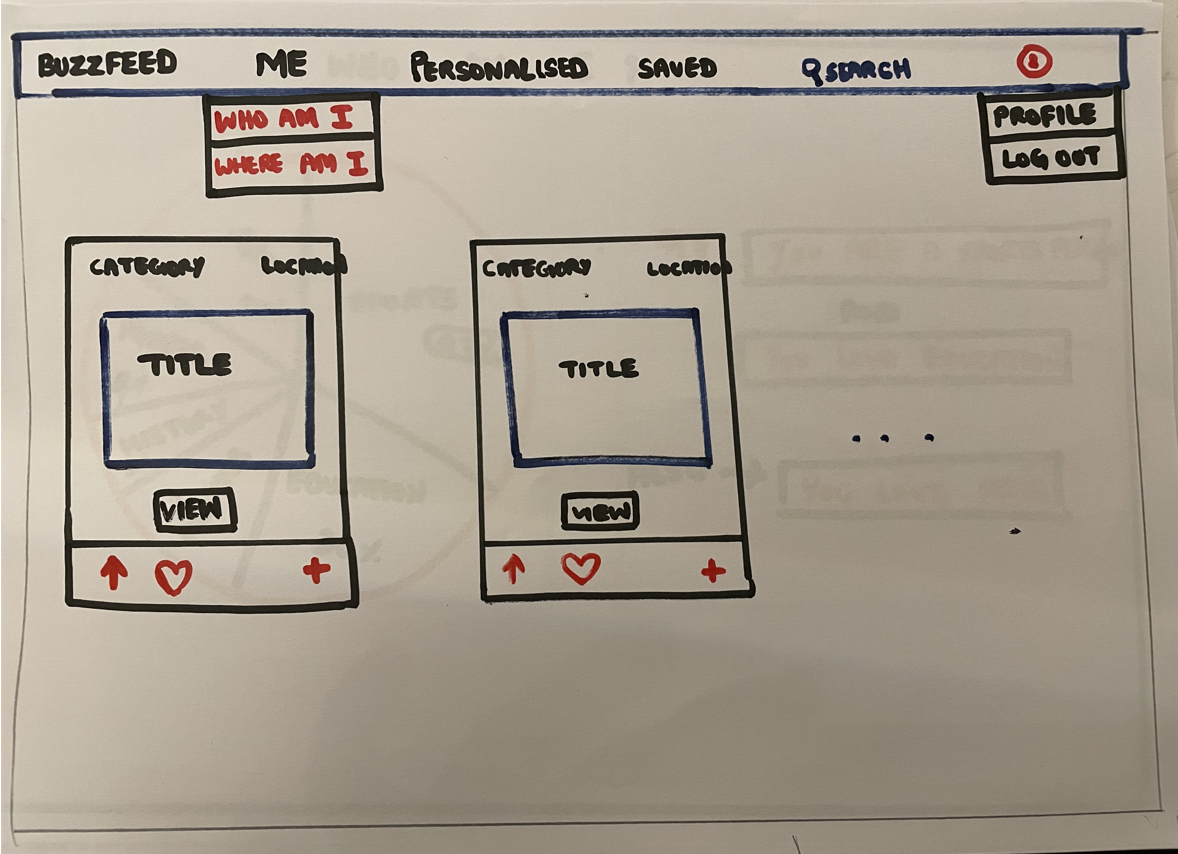
\includegraphics[width=\linewidth]{images/personalfeed.png}\par
    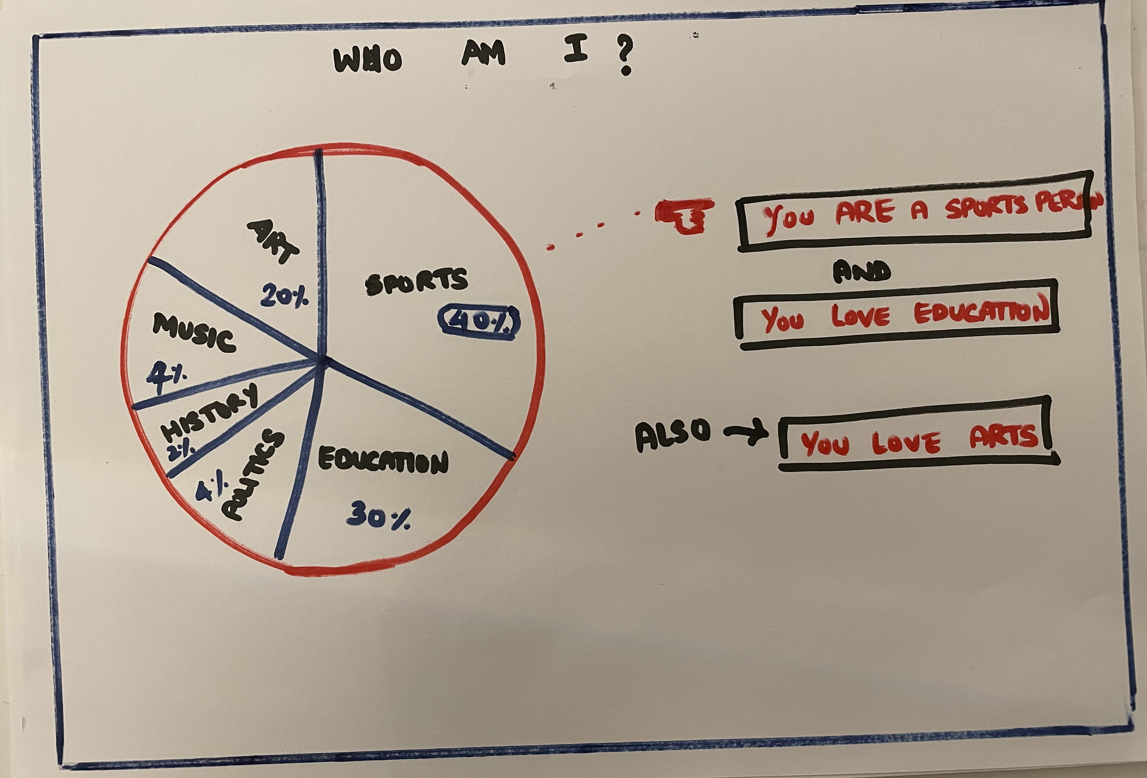
\includegraphics[width=\linewidth]{images/usercharts.png}\par
\end{multicols}
\centering \caption{Wireframe diagrams}
\end{figure}

    \item \textbf{H2 Database}\newline
    H2 is an open-source database written in java and hence it makes a very good combination with java springboot.
   
   \begin{figure}[h!]
   \begin{center}
       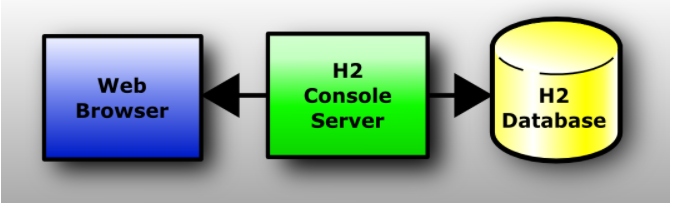
\includegraphics[scale=0.7]{images/h2.PNG}
        \centering \caption{H2 Database}

   \end{center}
   \end{figure}
    
    \textbf{Features of H2 Database}\newline
    H2 Database has the features compared against other databases which makes it more preferable to use.
     \begin{figure}[h!]
    \begin{center}
   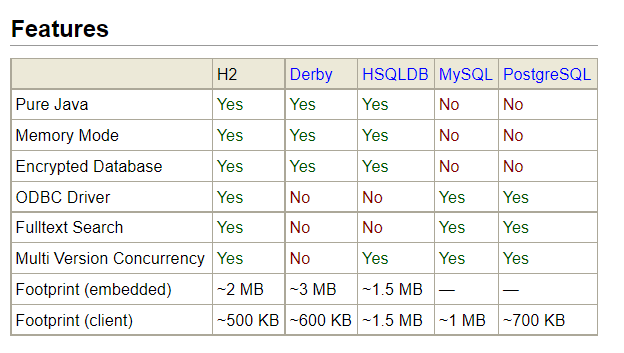
\includegraphics[scale=0.7,width=7in,height=4.5in]{images/h2features.PNG}
   \centering \caption{H2 Features}
    \end{center}
    \end{figure}
    The major reasons H2 database is used in our application are:
    \begin{itemize}
        \item \textbf{Java}: It is a Java open source database compatible with Springboot.
        \item \textbf{Embedded Persistent Database:} It supports several modes like embedded, in-memory and in both the modes it has persistent and in-memory databases. So, if we don't require to persist any changes to the database we go for in-memory or otherwise embedded database.
        This application works with Embedded Persistent database as there might be requirement for users to anytime update their details in their profile.
        \item \textbf{Encrypted security:} It has Encrypted security which makes the data secured.
        \item \textbf{H2 Console:} Additionally it has an option of H2 console which provides browser based access to the database.
    \end{itemize}   
    
        \item \textbf{Springboot Setup}\newline
        Springboot provides all the java application framework ready to start the development process. It comes with all the packages as separate dependencies which can be added anytime into the pom.xml which inturn builds the Maven and makes the dependencies available to use.
        
        Once the project is created with Java springboot the next step is to create Controller, Repositories and the Service class which makes the application run with respect to the Multi-layered Architecture. \newline
        
        \item \textbf{Angular modules}\newline
        Angular npm and node.js are installed and the project is started from scratch angular CLI command. 
        Angular is chosen because it supports code reusability, framework that supports component based development and supports many enhanced integration for appealing front-end UI components that can be used. \newline 
        
        Once the angular modules are installed the designs are implemented having wireframe diagrams as a reference.
        
      
        
        \item \textbf{Agile approach}
        
        The application is developed following agile standards which works very well with short-term standard software development.
        It is a results-focused development process which works adapting to the rapidly changing requirements. \newline
        There are many agile methodologies in software development process out of which the following are adopted in our application development cycle.
        
        \begin{itemize}
            \item \textbf{Working product:} The sprints are planned weekly and anytime the application is delivered or made available with a minimum viable functionalities ready to deliver.
            
            \item \textbf{Client Collaborations:} Meetings happened with the Professor and developer throughout the development.
            
            \item \textbf{Responding to Change:} The changing or updated requirements from Professors are considered and developed regularly to develop a complete product.
            
            \end{itemize}
    \end{enumerate}    
\section{Spring Boot Architecture}
    Springboot works in a layered architecture consisting of four different layers communicating directly above or below them. This can be run easily with the embedded tomcat server.
     \begin{figure}[h!]
    \begin{center}
          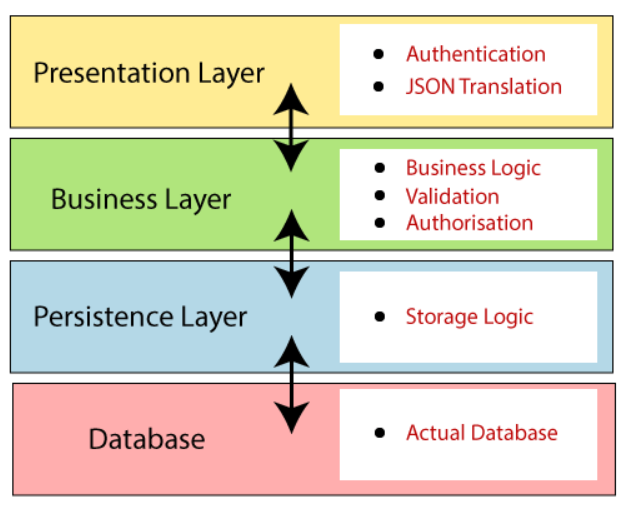
\includegraphics[scale=1]{images/springboot.PNG}
            \centering \caption{Springboot Architecture}
    \end{center}
    \end{figure}
    \begin{itemize}
        \item  \textbf{Presentation layer:} This is the front-end view where the application presents the features to the users and handles the http requests transferring to the business layer.
        \item  \textbf{Business layer:} This layer performs the business logic and handles the authentication and validation of application.
        \item  \textbf{Data Access layer:} This layer plays a key role in handling data to and from the databases which has a repository to do so.
        \item  \textbf{Database layer:} This is where the application data resides and all the operations like CRUD are performed\cite{www.javatpoint.com}.
  \end{itemize}
    \textbf{ \large Architecture Flow:}
     \begin{figure}[h!]
     \begin{center}
          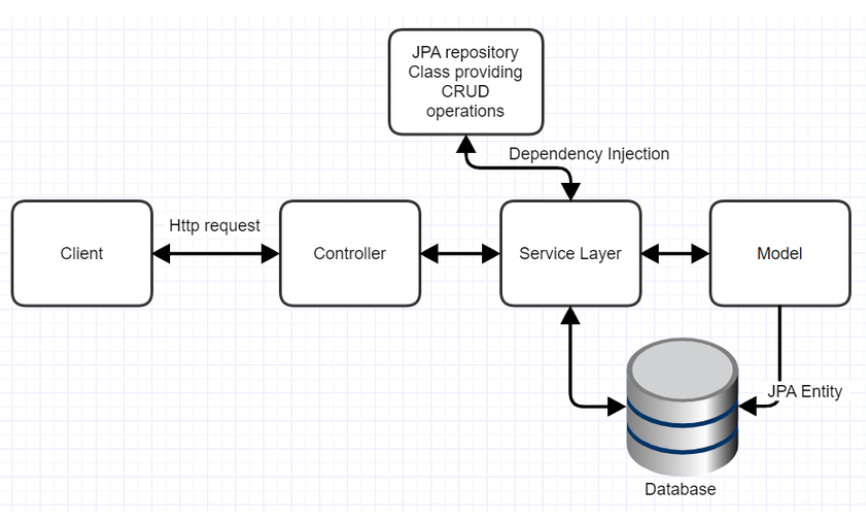
\includegraphics[scale=0.8]{images/Flow.PNG}
           \centering \caption{Architecture Flow}
    \end{center}
    \end{figure}
    \newline
    A Springboot application has a controller which process the http requests received from the client and it then interacts with the service layer where it does all the business logic for the application and data access or update using the repositories of the model \cite{springboot2020}. 
    
  \textbf{\large How It works in our Buzzfeed:}
  Sample architecture flow in our application is represented as follows:
   \begin{figure}[h!]
     \begin{center}
          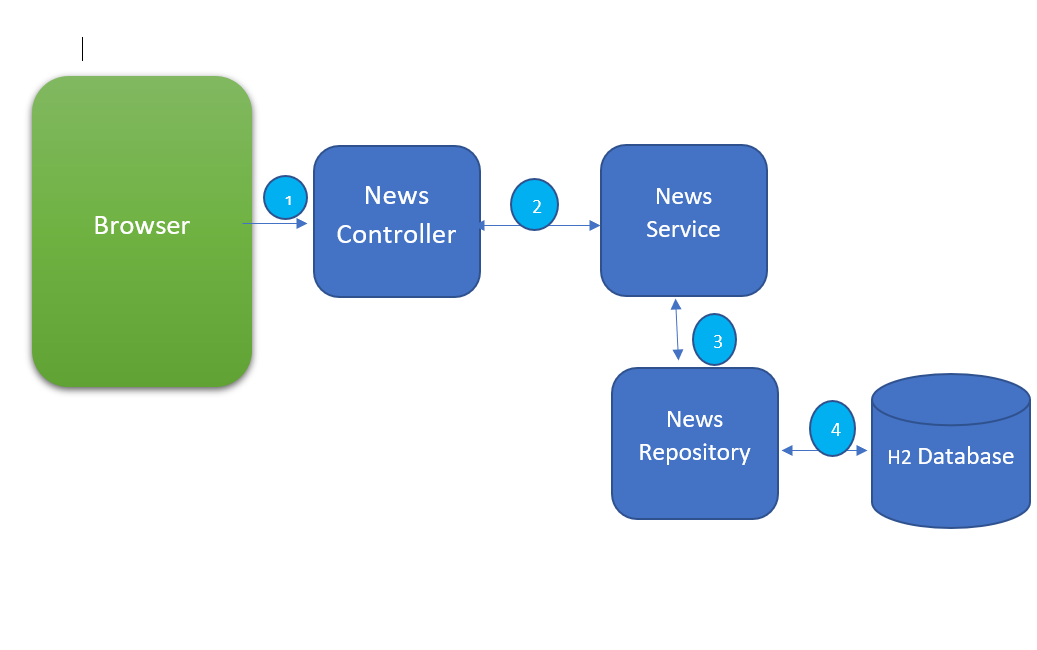
\includegraphics[scale=0.7]{images/example.PNG}
             \centering \caption{NewsFeed Server Flow}
    \end{center}
    \end{figure}
\begin{enumerate}
    \item Springboot News Controller receives the http requests from the frontend.
    \item The News Controller then process the requests to the News Service class which handles all the business logic and actions.
    \item The News Service class then process the data from the database or updates the data to the database through the database access layer called New Repository.
    \item The H2 Database stores the data and handles the data storage and updates if any. It is embedded Persistent database in our application so it can effectively persist data in case of changes and it is immediately available.
\end{enumerate}
 
 \section{Object Oriented Design}
 
      
             \subsection{Use Case Diagram}
            Use Case diagrams is the visual representation of system requirements. It gives a glimpse of what the system is intended to do to the stakeholders and the users of the system. Here the main actor is the user in various forms and an external Mahout recommendation system which interacts with the system. The below diagram gives an idea of what the system does in brief.
             \begin{figure}[h!]
                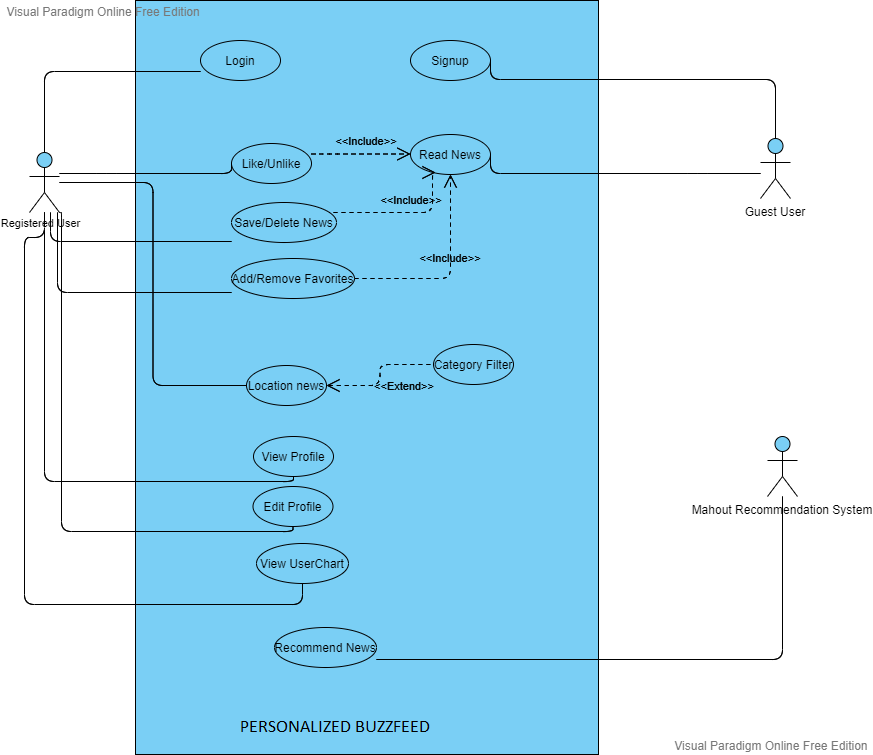
\includegraphics[scale=0.9]{images/Buzzfeed.vpd.png}
                 \centering \caption{Use Case Diagram}
            \end{figure}
      
           \subsection{Class Diagram}
            Below Class diagram represents the static view of the application and it has attributes and operations which represents the structural and behavioral features of the application.
             \begin{figure}[h!]
             \begin{center}
             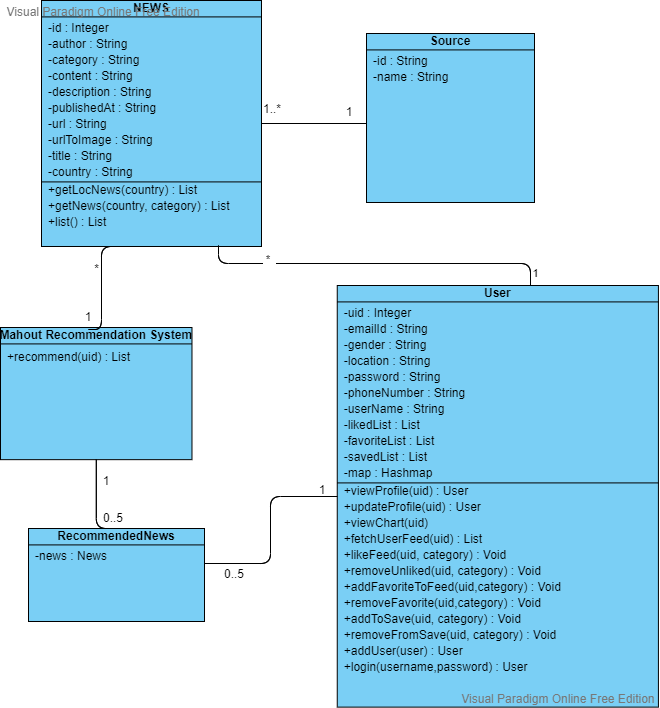
\includegraphics[scale=0.7]{images/Classdiagram.png}
              \centering \caption{Class Diagram}
             \end{center}
              \end{figure}
              
\section{Database Design}
      The database design for the application is represented as :
       \begin{figure}[h!]
             \begin{center}
             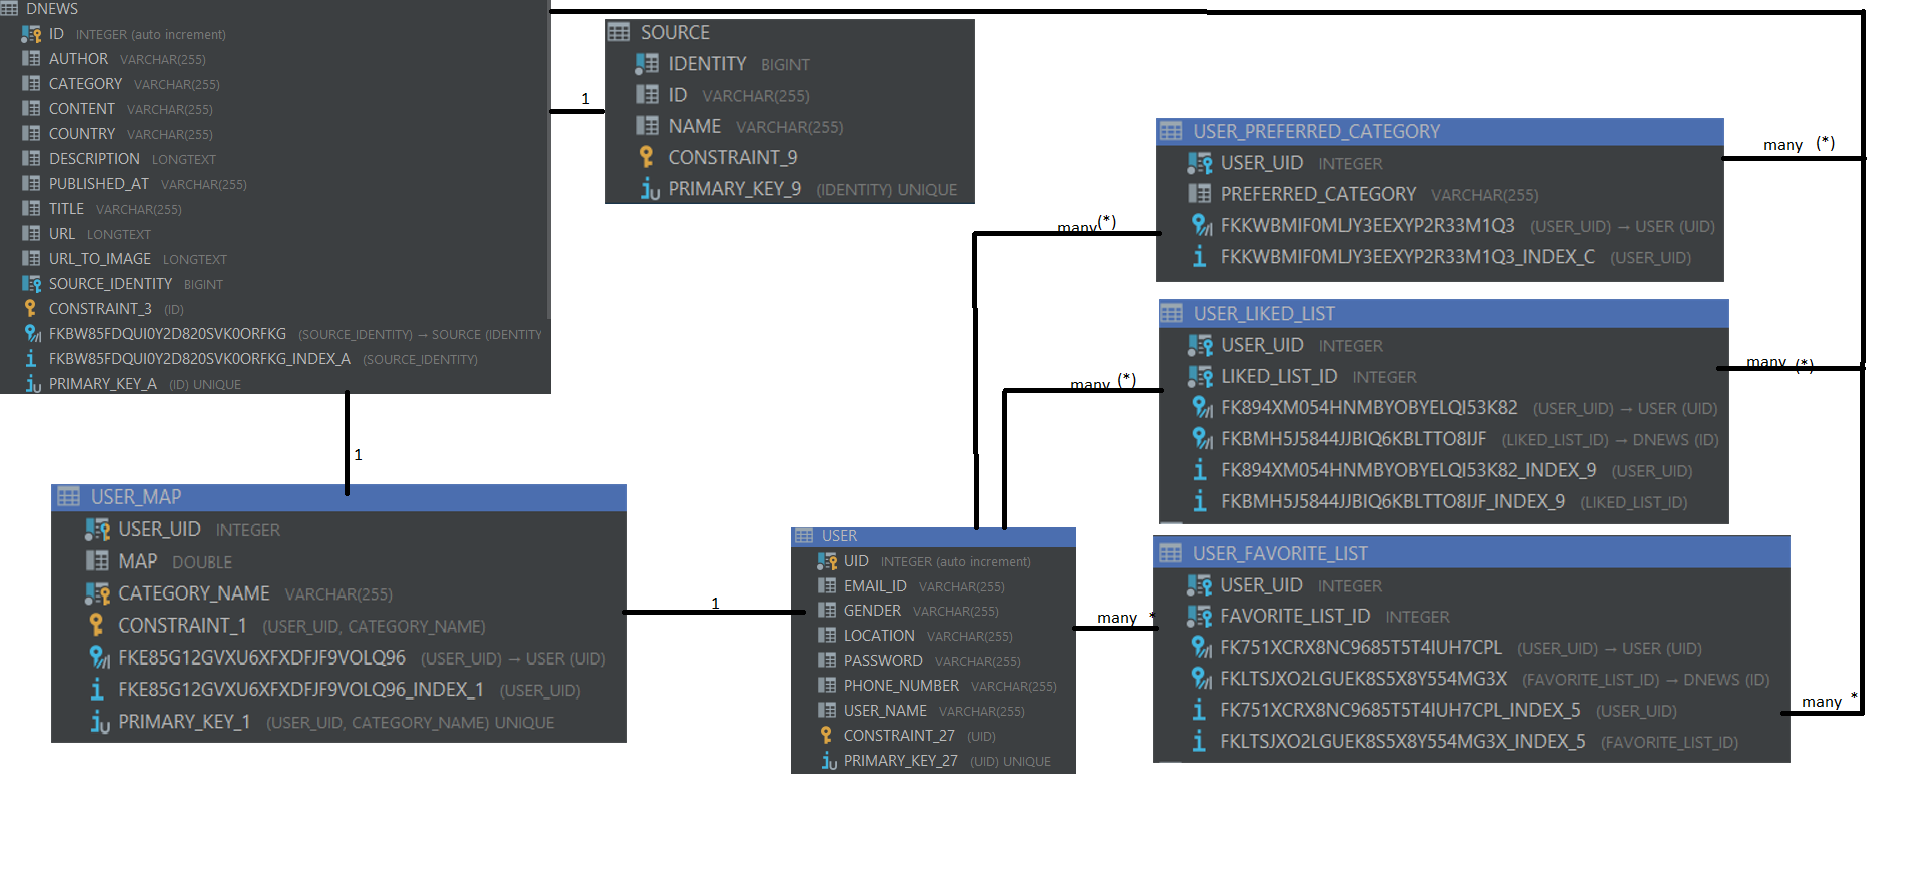
\includegraphics[scale=0.45]{images/DatabaseDesign.png}
              \centering \caption{Database Design}
             \end{center}
              \end{figure}
\section {Application Design and Workflow}

\subsection{News Dataset}
The first and the foremost activity for this application is to gather the right dataset that is required to accomplish the product. There are many datasets and third party service APIs that provides the news data that are required but there were certain limitations in the necessary fields that out news model needs.

\textbf{\Large NEWS API}\newline
There is a third party rest API service called - 'NEWS API' which provides live news articles throughout the globe.
It is accessible through - https://newsapi.org/ \newline
The application sticks to the database data for news data even when we get the live news without any restrictions from NEWS API service is to stay in some safe zone for the final project presentation and avoid any dependencies in order to avoid any case of unexpected issues of loss of data at the time of presentation \cite{newsApi}.\newline

\textbf{Why NEWS API:}\newline The News Api is chosen as the news dataset for our project as we require few major fields like category, url, url Image and ccountry details to present the news to any news readers in our application.
And most importantly there is a requirement to classify the articles based on country and category and these fields can be made available with the news api request. Hence we decided to go with News API service. \newline

Let's see the structure of news api request and response and how it can be made useful for us.\newline
\textbf{NEWS API Request:} \newline
 The NEWS API request can be obtained from https://newsapi.org/v2/top-headlines
 which will result in all country top news that can be processed. \newline
The is carried out for few countries and categories from the NEWS API and then processed for the response. \newline
\textbf{Request Parameters: }\newline
 The request parameters we have chosen for our application includes the following: 
 \begin{itemize}
     \item \textbf{APIKEY:} This is more important and unique for individual users and allows access to the news api. 
     \item \textbf{country:} The two-letter country code for whichever countries we need news.
      \item \textbf{category:} The category news we may be interested in can be selected from the available set of categories list: Business, technology, entertainment, health, sport,general and science.
 \end{itemize} 

\textbf{NEWS API Response: }\newline
    The NEWS API Response data has many fields which makes it more flexible for our application. 
  \begin{itemize}
     \item \textbf{Title:} The headline for the news.
     \item \textbf{description:} Descriptive information about the article to know more details.
     \item \textbf{URL:} To navigate to the respective url for the news publications to go through the whole article.
     \item \textbf{URL Image:} To have the respective images with the news article that makes more sensible.
     \item \textbf{Source:} The valid source information for the article who has published the news.
     \item \textbf{Published At:} The published time and date for the article by the source.
     
     The response does not have country and category fields directly available but appended to the items in the database.
     
  \end{itemize}  
 
\subsection{News Feed}
 The next phase of the application is to present the news to the guest users to view the articles but to like or add them to favorites they need to have a valid login credentials and logged into the application.
 
 \textbf{NEWS FEED Design:}
    News articles is now available on the database. The only operation we do here is to just fetch or read the news for a guest user.  
    \begin{figure}[h!] 
  \begin{center}
          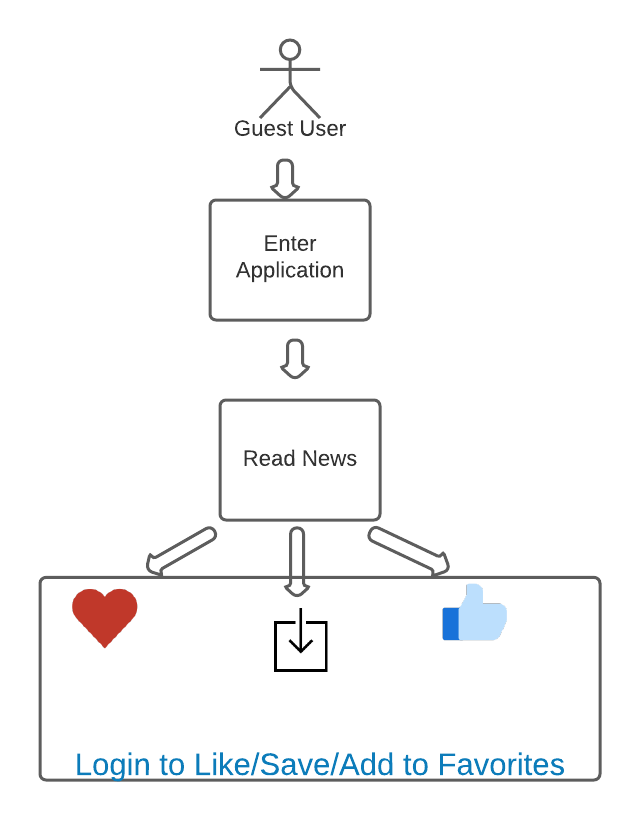
\includegraphics[scale=1]{images/GuestUser.png}
        \centering \caption{Guest User}
    \end{center}
    \end{figure}
The Guest user access is controlled to view just view and read the news and restricted from interactions with the article as they interactions cannot be monitored for personalization. \newline

 
\subsection{Registration and Login}
   
   \begin{enumerate}
{\bf \item  Add User Profile}
    \begin{itemize}
       \item \textbf{User Registration:} The users are requested to give some basics information about them to derive their interests from their context details for setting up their initial preferences. This user details page is primarily important for 'User Profiling'.
       
       \item\textbf{ User Login: }
        Users login module works with JWT authentication mechanism to allow users to login and view and interact with the application. \newline
         \end{itemize}
       \textbf{ Spring Security and JWT Authentication}
        \begin{figure}[h!]
       \begin{center}
          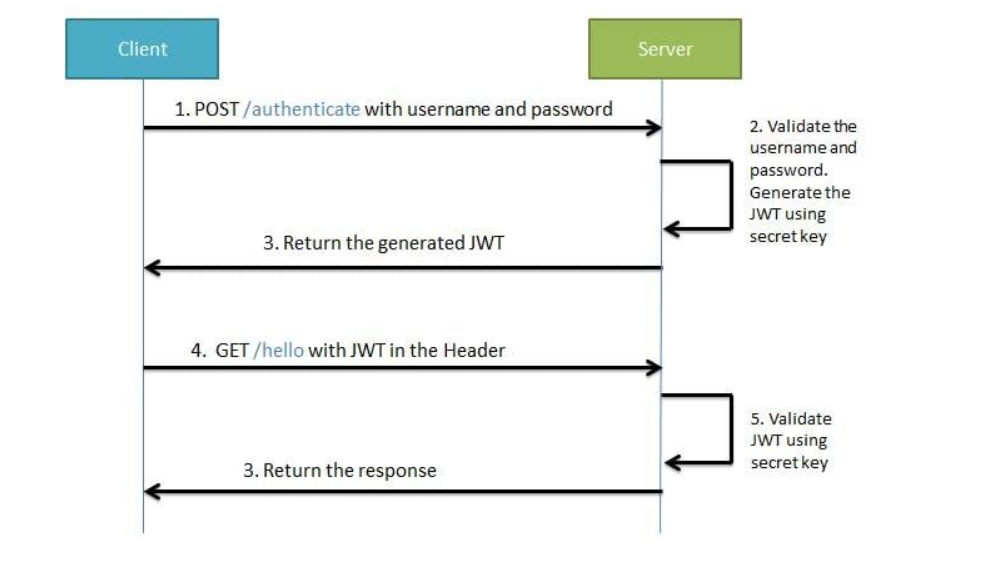
\includegraphics[scale=0.8]{images/JWT.PNG}
            \centering \caption{JWT Authentication}
    \end{center}
    \end{figure}
        This module is designed inline with the Spring Security concepts which authenticates the user with their login credentials.
        On valid Authentication with the username and password, the server responds to the client with a valid\textbf{ JWT token} generated with the user details.
        Upon receiving the JWT token, the client has to send all the http requests with the authentication header in bearer token form otherwise it the request would be rejected by the server.\newline 
        This way it secures all the http requests and response in Spring Security application \cite{jwt2020}.
    
    \textbf{Spring Security Architecture}
     \begin{figure}[h!]
        \begin{center}
          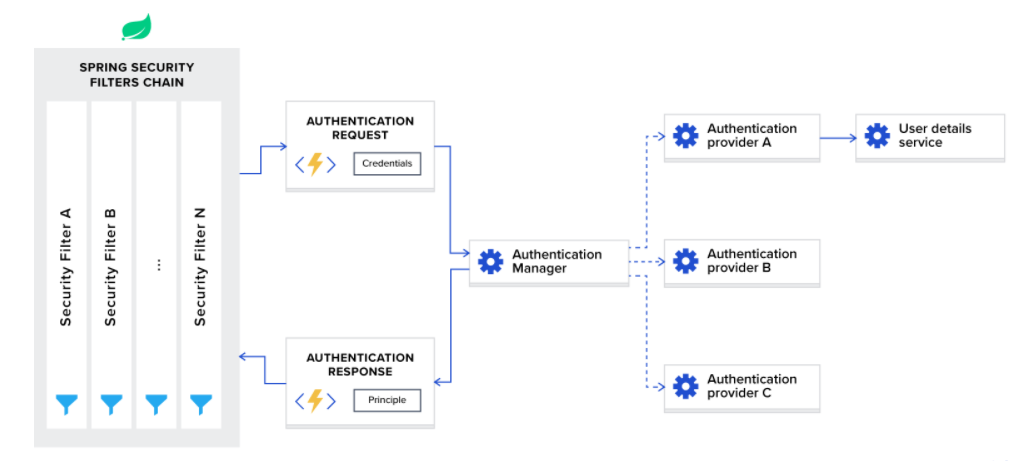
\includegraphics[scale=0.8]{images/springsecurity.PNG}
            \centering \caption{Spring Security}
    \end{center}
    \end{figure}
\textbf{Authentication manager:} \newline
    Spring Security works with Authentication manager processing the http requests and the response.
 \textbf{Authentication Providers:} \newline   
    Authentication manager has multiple Authentication providers which process different types of authentication services. This is an interface which has a function called 'authenticate' which authenticates the user upon request.
    
     \textbf{User Details Service Class:} \newline   
     Additionally on valid authentication, it is necessary to generate JWT token with the username. Hence to achieve this we implemented \textbf{UserDetailsService} class in our application which loads user data with the username using the method loadByUsername. This helps in generating the JWT tokens with user claimed details.
    
   

       {\bf \item  View User Profile:} \newline
        Once the user is logged into the application, he lands in the user details page where he can view his/her profile details given during the registration process. This is processed as GET REST API call to the backend.
        
        {\bf \item  Update User Profile :}\newline
        The logged in user can also update his user profile from the client side anytime and view the updated details of his profile. This is processed as UPDATE REST API call to the backend.

 \subsection{User Personal Feed}  
 User personal feed loads different content for each user based on user's likes and interests. It analyses individual's interests with the static and dynamic states and decides the overall weightage for the preferences of categories for each user and loads them respectively.\newline
 Here is where personalization comes into picture. Personalization plays a key role in this application and configured in two different ways as mentioned.\newline
 
 \textbf{ User Category Map:}
 Each user on signup is assigned a Hashmap which maps users preferred category and their respective weight. So this keeps track of the users most favorite category based on weight.
 
 \begin{itemize}
     \item\textbf{ Contextual Personalization:} Achieved with the User Profiling. Here the selected preferences during the signup and the location are considered.
     The selected categories on signup will be added \textbf{+2.0 }weights and the rest\textbf{ 0.0 }. This map stores individual users category weightage. This is performed each time when a new user is created.\newline
     The location preference is used in visualized personalization context which comes in a later view.
      \item\textbf{ Behavioral Personalization:} This works understanding the users varying interests everytime and keeps it updated in the category map on change.
      It analyses the users likes, dislikes, favorites, saved news and understands the preferences implicitly and maps the preference weights accordingly. \newline
      So, lets discuss how it judges the various interactions programmatically in brief with a pseudocode following the explanation.
      
      \begin{enumerate}

{\bf \item Likes:} 
The likes are identified with a filled thumbs-up icon and everytime the users like any article the respective category is identified and that category weight is increased by \textbf{+1.0} each time. 
This way it keeps the liked category into account and the user's category-map is updated.
{\bf \item Dislikes:} 
The likes are identified with an unfilled thumbs-up icon and everytime the users like any article the respective category is identified and that category weight is decreased by \textbf{-1.0} each time. \newline
 \hspace*{1cm}This way it keeps the liked category into account and the user's category-map is updated. This is marked a lower weight as the likes and dislikes sometimes are random hits based on the story or the article and cannot completely assure the interest rate.\newline
\textbf{Like Zone:}
Also, the associated liked articles are mapped to a list and made available for users anytime to re-visit their liked ones.\newline

{\bf \item Favorites:} 
The favorites are denoted by a filled heart icon and the user's favorite article's category is identified and the respective category weight is increased by \textbf{+3.0}.

{\bf \item Unfavorites:} 
The favorites are denoted by an unfilled heart icon and the unfavorite article's category is identified and the respective category weight is reduced by \textbf{-3.0}. \newline \hspace*{1cm}This is marked a higher weight compared to other interaction as the favorites explicitly states they are the most interested and remain almost the same. \newline
\textbf{Favorite Zone:}
Similarly users favorite articles are monitored and stored in a separate view for the users to revisit and go through their favorites anytime.\newline

{\bf \item Saved Articles:} 
The users are allowed to save their news articles to make them available anytime for later read. This is a similar functionality that we have in many applications like Read Later and Watch later items. This helps the users to keep track and not miss the articles from reading at a later time.
This is highlighted by a filled download icon and the weight associated with this option is \textbf{+2.0} for the respective category on save.

{\bf \item Delete Saved:} 
    This allows the user to remove any article from saved list once they read through the article and there is no purpose having it in the saved items or read later items anymore.
    The respective added weight while saving is decreased here to maintain the consistency of the category preferences\newline
\textbf{Read Later:}
As mentioned there is a separate view for read later items to make it easy for users to know where exactly the saved items are and help them read and delete anytime based on their interests.\newline

      \end{enumerate}
 \end{itemize}
   \end{enumerate} 
\textbf{Automated Personalization:}\newline
The above theoretically described personalization is achieved using a custom-designed algorithm called\textbf{ ‘Weight-Map’ Algorithm}.

\textbf{Weight-Map Algorithm:}\newline Weight Map Algorithm builds user Personalization programmatically based on above mentioned factors or user engagements.
Each user engagement is counted and assigned respective weights as described above.
The algorithm is named as 'Weight-Map' algorithm because a hash map is created for each user which maps users category based weights in the backend.

\textbf{Similar Existing Algorithm:}
Facebook determines the personalization of feeds based on an algorithm called 'Edge Rank' Algorithm\cite{geeksforgeeks2018}. This is a rank-based approach considering three major factors: Affinity Score, Edge Rank and Time Decay. These factors ranks and decides the order of appearance of stories in the user's newsfeed.\newline

The updated facebook algorithm works based on the likelihood of the user interatcions with the post. This is a complex algorithm which has to cross four systems.
\begin{enumerate}
    \item \textbf{Inventory :} This is the initial phase where the facebook decides what all contents to load for any user based on his affinity which means the close relationship graph.
    \item \textbf{ Signal :} This phase has to approve the content based on various assessments like type of feed, whom and when the content was posted, the likes, shares,comments and all other factors and given \textbf{weightage}.
    \item \textbf{Predictions:} This phase predicts how far the respective user might like the posts based on his previous behaviour\cite{WebFX2021}.
    \item \textbf{Score:} The above two phases are combined like the predicted story and the respective weight for that story are combined and assigned a relevancy score which helps in fetching the news feed sorted in descending order.
\end{enumerate}

\textbf{Comparison  - Similarities and Differences To Weight-Map Algorithm: }
\begin{enumerate}
    \item \textbf{ Phase 1: } \newline
 Weight-Map algorithm works in a simplified pattern taking all the contents at the first phase.
     \item \textbf{ Phase 2: } \newline
 The second Signal phase works bit differently. Instead of evaluating each content, we assign weights for user interacted content's category everytime the user likes, saves or add the news to favorites. Actually this is the third phase of predictions according to facebook algorithm which is our only filtering mechanism and scoring method for assigning weights.\newline For example, The user likes certain article, then the category weight for that article increases by +1.0 and the vice-versa.
     \item \textbf{ Phase 3: } \newline
This is the final phase where we filter based on weights or score assigned to categories interested for each user. Each user will have a category-weight map assigned in previous phase which is sorted in descending order and then based on more range of weights to load respective number of articles.\newline  For Example. category score more than 50, loads 20 articles from that category and for a lesser score the limits decreases.
 Then with the overall category weightage we provide the users with their personal feed.

\end{enumerate}
\textbf{Visual Representation of Algorithm:}
The below figure helps us to understand more clearly on how this algorithm works.
 \begin{figure}[h!]
\begin{center}
              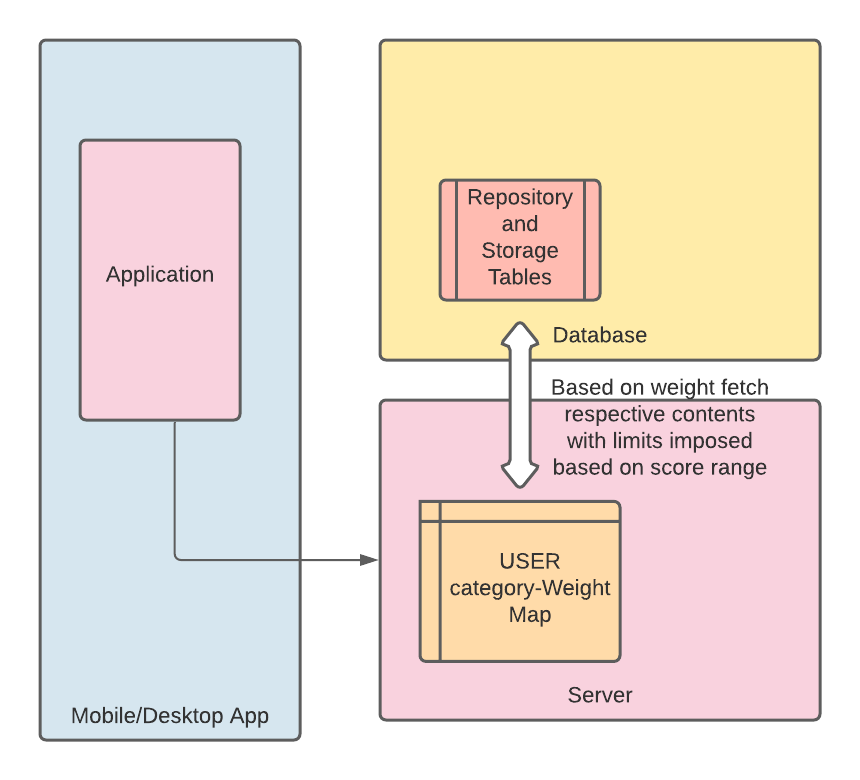
\includegraphics[scale=1]{images/WeightMap Algorithm.png}
                 \centering \caption{Weight-Map Algorithm Flow}
\end{center}
\end{figure}
\textbf{Pseudo-code of Weight-Map Algorithm:}
\begin{lstlisting}
User register: 
	if preferredcategory in categoryList:
		category-map.weight = 2.0
    else	
		category-map.weight = 0.0
    Add user with cmap
Monitor Actions:
  if(logged in):
	if click(Like): 
	   if(liked):
    		fetch category for this feed
		    Add category-map.weight - 1.0
        else:	
    		fetch category for this feed
    		Add category-map.weight + 1.0

	if click(Favorites): 
	    if(favorite):
    		fetch category for this feed
    		Add category-map.weight - 3.0
        else: 	
    		fetch category for this feed
    		Add category-map.weight + 3.0
	
	if click(Save): 
	    if(saved):
    		fetch category for this feed
    		Add category-map.weight - 2.0
        else: 	
    		fetch category for this feed
    		Add category-map.weight + 2.0
  else:
    print(Login to personalize!)
\end{lstlisting}

And to prevent the userfeed from overload with all news of a particular preferred category, the application imposed limits on the results to load the news collection from specified category based on its weight. More the range of weight, more are the number of results from that particular category and vice-versa.
This enables to prioritize the top category preference and load them more instead of loading everything equally.

\begin{lstlisting}
User-feed:
     	fetch sorted category-map based on weight
	for sorted category in category-map
		if(weight > 50)
			fetch top 20 newsfeed on this category
 		if(weight > 10)
			fetch top 12 newsfeed on this category
		if(weight > 5)
			fetch top 8 newsfeed on this category
		else
			fetch top 5 newsfeed on this category

\end{lstlisting}

\subsection{Visualization}
Visualization is accomplished by a special library called amcharts which gives sensational maps and charts which are effective for locating the news around the globe and understanding the user chart data.

Visualization is applied in two areas in our application. 
\begin{enumerate}
    {\bf \item User Charts:}
     User charts are visible in the user profile view where every user will be able to see their category chart which shows them their most favorite category and the overall percentage of interests he expressed while reading through the news articles in the application for all the available categories.\newline
     This is represented in terms of pie-chart which shows the category-name and rate of interests in percentage along with the number of articles which made the figure.
     
    \textbf{Pie-charts:}
    Pie-charts represents a part-to-whole relationship. Every piece or slice of a pie-chart represents one component which together contributes the whole\cite{amcharts_2018}.\newline
    \textbf{Why Pie-charts:}
    Pie-charts help clearly help us to understand how much each category contribute in a user's interests because pie-charts are best used in case of explaining and understanding part-whole relationship. Also, it is bit more attractive than simple column or bar charts in a way hence the choice of pie-charts.\newline
   \textbf{ Pre-requisites:}
   We installed the external library -\textbf{ @amcharts/amcharts4} to have the basic functionalities from amcharts 4.
   Once integrated the amcharts, we can extend to any additional pluggins which we require in future.\newline
   To achieve amcharts pie-charts we required two modules - \textbf{am4core and am4charts} which were installed.
   
     {\bf \item Globe View:}
     Another area where we have the visualization is the map or the globe view in the application where it projects a map in orthogonal projection.\newline
     \textbf{ Pre-requisites:}
      For acquiring the maps, we need \textbf{am4maps} module which gives the globe view and we can make this to appear in any projection like a globe or a flat map.\newline
      \textbf{Why Orthographic projection:}
      We have chosen \textbf{Orthographic projection }in this application which is a globe structure because it is more interactive and looks appealing to the users as it keeps rotating around which makes it lively.\newline
      
      Here is how it looks when projected:
       \begin{figure}[h!]
      \begin{center}
         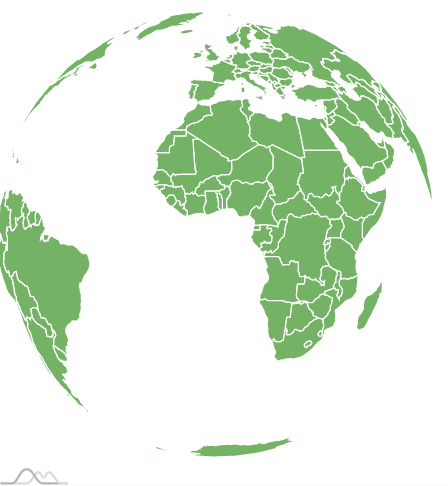
\includegraphics[scale=1]{images/globe.PNG}
          \centering \caption{Amcharts Map}
      \end{center}
      \end{figure}
       \textbf{How it is designed to help us:}\newline
     \textbf{ Visual Country Filter:}
      This view of globe allows users to chose which country's news they would like to read through anytime. This helps in filtering the news for each users preferred country.\newline
      \textbf{Category Filter: }
      At the same time, when the users prefer to know more about each country specific category news, the application gives them another option to select any category they need from a list of categories which again filters selected category data for selected country.\newline
         \textbf{ Combined Filters:}
      Thus two filters are applied on user's preference.
      So, users can read any country news and any category news and compare the category news data against any other country if required.\newline
       So, technically the combination of filters is achieved using \textbf{Behavioral subject} in angular. This helps in retaining the category selected for change in country and change the category selection only on subscription.\newline
       \hspace*{1cm}\textbf{For example:} When the user selects 'Australia' the application loads the Australia country results with 'All' categories selected. When the user changes the category to 'Sports' the user will be able to look specifically Australia's Sports data and change to any other category or country as preferred. \newline
        \textbf{ Personalized Visualization:}\newline
      Initially to make it more personalized, we load the \textbf{user location} by default with \textbf{'All'} categories loaded in the results. 
      This allows the user to open the view and have a look at his/her country data and option to see any category data for the location.
      
     \textbf{ Whom It helps Mostly:} It is mostly helpful for journalists or news organizations who compare news against countries and want to understand the worldwide news in compare and contract approach.
     Also, it obviously helps the general users who are interested to know more information anytime.
    
\end{enumerate}

\subsection{Recommendation}
Recommendation is provided for each user based on user's interests rate compared against other users who have similar interest pattern.\newline
\textbf{Mahout Recommendation System:}
This is achieved using \textbf{Mahout Recommendation system} which handles real-time users interests data and recommends articles based on Collaborative Filtering algorithm. It is chosen because it supports different approaches for Collaborative filtering both item-based and user-based and also highly scalable for large datasets\cite{mahout_2012}.
For Example, Amazon and Netflix recommendation systems.

\textbf{Recommendation System Architecture:}
Recommendation works in several stages as follows:
 \begin{figure}[h!]
\begin{center}
    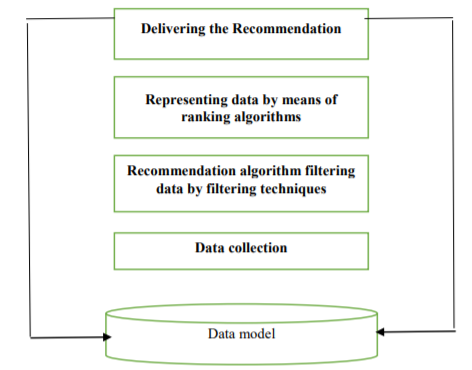
\includegraphics[scale=1.5]{images/recommendation.PNG}
     \centering \caption{Recommendation Architecture}
\end{center}
\end{figure}

\textbf{Proposed Approach - User Based Recommendation:
}
User-based approach is chosen for this application and it works on the concept that users who have similar interests will be interested towards similar categories\cite{madhushree2016}.\newline
Algorithm works in three steps\cite{madhushree2016}.
\UseRawInputEncoding
\begin{lstlisting}
For every item I that u has no preference for yet
For every other user v that has a preference for i
    Compute a similarity s between u and v
Incorporate v’s preference for I weighted by s to avg
Return the top items, ranked by weighted average
\end{lstlisting}

\textbf{Explanation of Algorithm:}
 \begin{enumerate}
     \item 1. Find user u with no preference for item say. i
     \item 2. Find other users v who has preference towards i and have similarity model between  u and v
     \item 3. Compute average for the preference for items and recommend items with top weight.
 \end{enumerate}
 
\textbf{How does it work for Buzzfeed:}
Buzzfeed also works out this algorithm in three stages except that incorporating weight is not necessary here as we have them pre-calculated for every user in user-category map. \newline
\textbf{Recommendation Input Data:} The input data is obtained from user-category map stored in database table where we have the user category and respective weights for every user which we convert to csv files for Recommendation process.

\textbf{How it Works:} 
Let's discuss the working process with an example. When user 'u' has more interest weights for categories 'Sports' and 'Science' and there are other similar users with more which is around similar weight as of 'u' for 'Sports', 'Science' and additionally has more weight for other category 'Club', so the user 'u' is recommended with some items in 'Club' which might sound interesting for the user.\newline
\textbf{Observed Limitation:}
This is more related when the there are more number of categories and users are not sure which one they find to read sometimes. For our application, we have less number of categories due to some dataset limitations but it helps in understanding how it works clearly.
